We define a \textit{chessboard polygon} to be a polygon whose sides are situated along lines of the form $ x = a$ or  where $ a$ and $ b$ are integers. These lines divide the interior into unit squares, which are shaded alternately grey and white so that adjacent squares have different colors. To tile a chessboard polygon by dominoes is to exactly cover the polygon by non-overlapping $ 1 \times 2$ rectangles. Finally, a \textit{tasteful tiling} is one which avoids the two configurations of dominoes shown on the left below. Two tilings of a $ 3 \times 4$ rectangle are shown; the first one is tasteful, while the second is not, due to the vertical dominoes in the upper right corner.

\begin{center}
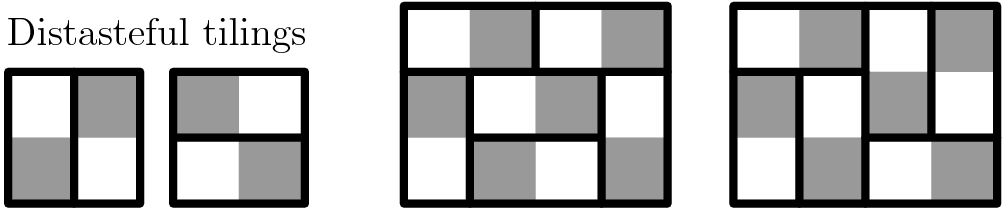
\includegraphics[width = 100.4mm]{img/fig0.png}
\end{center} a) Prove that if a chessboard polygon can be tiled by dominoes, then it can be done so tastefully.

b) Prove that such a tasteful tiling is unique.